\section{Final Velocity Model}
%It is possible to draw a block diagram for the drivetrain, from the motor torque to the vehicle's velocity with \eqref{eq:TransferFunctionTorqueToVelocity}. Furthermore, the motor needs the produced angular velocity to get affected by the load, i.e. drivetrain. The angular velocity was found in \eqref{eq:BlackBoxGearNewtonLaplaceNew}.

\begin{figure}[H]
	\centering
	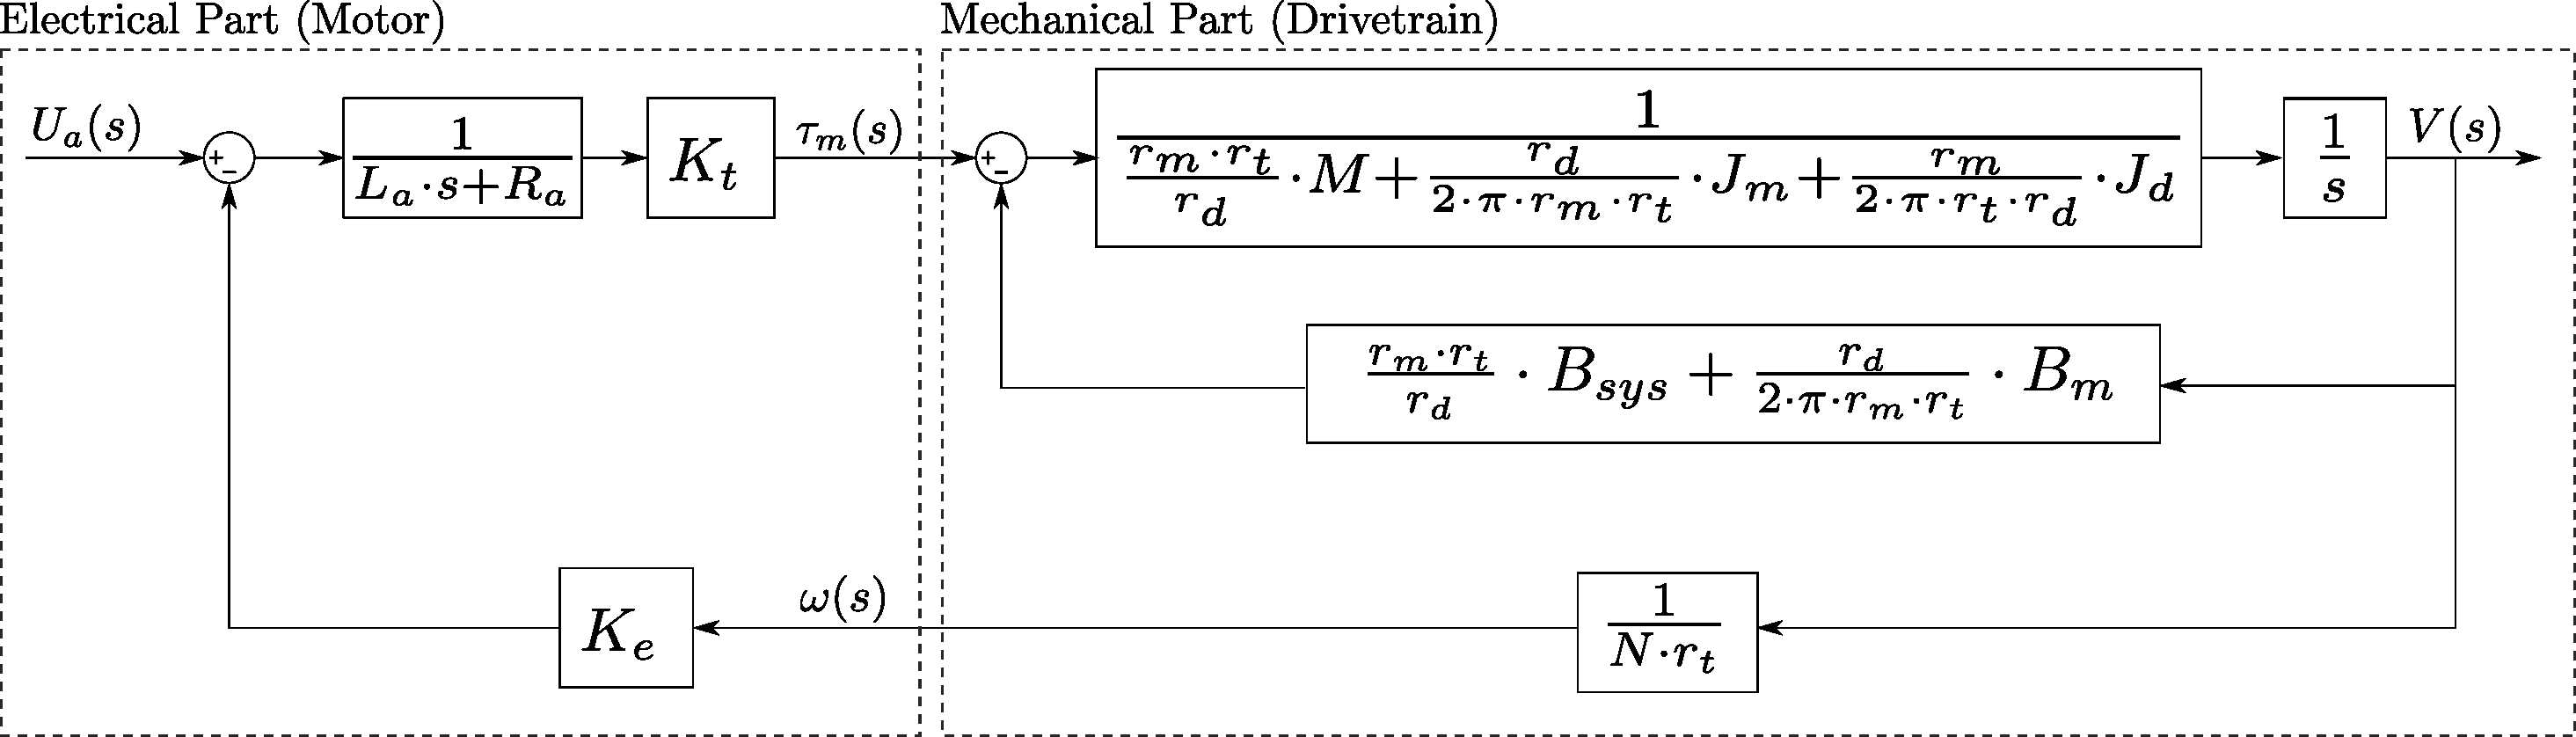
\includegraphics[scale=.28]{figures/totalVelocityModelDiagramComplicated.pdf}
	\caption{A block diagram of the combined drivetrain}
	\label{fig:BlockDiagramDrivetrain}
\end{figure}

%A block diagram describing the drivetrain has been built. In the following section the drivetrain's block diagram is combined with the motor's block diagram, seen in \figref{fig:motormodelBlock}.